{\textbf{{1. IPv6的首部格式}}}

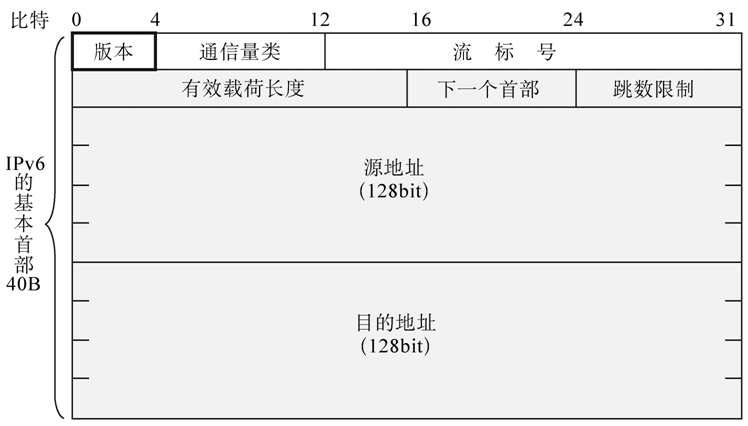
\includegraphics[width=3.33333in,height=1.89583in]{png-jpeg-pics/AB77CD74448F1E8AD96A989EBCB203E3.png}

\textbf{1)版本(version)。}占4位,它指明了协议的版本,对于IPv6,该字段总是6。

\textbf{2)通信量类(Traffic
Class)。}占8位,这是为了区分不同的IPv6数据报的类别或优先级。

\textbf{3)流标号(Flow
Label)。}占20位,``流''是互联网络上从特定源点到特定终点的一系列数据报,``流''所经过的路径上的路由器都保证指明的服务质量。所有属于同一个流的数据报都具有同样的流标号。

\textbf{4)有效载荷长度(Payload
Length)。}占16位,它指明IPv6数据报除基本首部以外的字节数(所有扩展首部都算在有效载荷之内),其最大值是64KB。

\textbf{5)下一个首部(Next
Header)。}占8位,它相当于IPv4的协议字段或可选字段。

\textbf{6)跳数限制(Hop
Limit)。}占8位,源站在数据报发出时即设定跳数限制,路由器在转发数据报时将跳数限制字段中的值减1。当跳数限制的值为零时,就要将此数据报丢弃。

\textbf{7)源地址。}占128位,数据报的发送站的IP地址。

\textbf{8)目的地址。}占128位,数据报的接收站的IP地址。

\textbf{{2. IPv6的3种地址类型}}

\textbf{1)单播。}传统的点对点通信。

\textbf{2)组播。}数据报交付到一组计算机中的每一个广播可看作是组播的一个特例。

\textbf{3)任播。}其目的站是一组主机,但数据报在交付时只交付给其中一个,通常是距离最近的那个。

{\textbf{3. IPv6的地址表示法}}

为了使地址简洁,{\textbf{通常采用冒号十六进制法表示IPv6地址。}}它把每16bit用一个十六进制数表示,各值之间用冒号分隔,如68E6:8C64:FFFF:FFFF:0111:1180:960A:FFFF。

通常可以把IPv6地址缩写成更紧凑的形式。当16位域的开头有连续的0时,可以采用缩写法表示,但在域中必须至少有一个数字,\textbf{{如可以把地址5ED4:0000:0000:0000:EBCD:045A:
000A:7654缩写成5ED4:0:0:0:EBCD:45A:A:7654。}}

当有相继的0值域时,还可以采用双冒号表示法进一步缩写。这些域可以用双冒号(::)。但要注意,{\textbf{双冒号表示法在一个地址中仅可以出现一次}},因为0值域的个数没有编码,需要从指定的总的域的个数中推算。这样,前述示范地址可以被更紧凑地书写成5ED4::EBCD:
45A:A:7654。
